% Generated Stage 3 integration deck.
\documentclass[aspectratio=169]{beamer}
\usepackage{amsfonts,amsmath,amssymb,booktabs,graphicx}
\makeatletter
\def\input@path{{styles/}}
\makeatother
\usetheme{sintef}
\titlebackground*{assets/background}
\usepackage{tikz}
\usetikzlibrary{arrows.meta,positioning,calc}
\newcommand{\StageThreeNode}[5]{\node[anchor=north west,align=#4,text width=#3\paperwidth,inner sep=0pt] at (#1,#2) {#5}}
\newcommand{\StageThreeBox}[4]{\draw[rounded corners=1.5pt,line width=0.7pt,draw=maincolor!75,fill=white] (#1,#2) rectangle (#3,#4)}
\newcommand{\StageThreeArrow}[4]{\draw[-{Latex[length=2mm]},line width=0.8pt,draw=maincolor!75] (#1,#2) -- (#3,#4)}

\setbeameroption{hide notes}
\bibliographystyle{unsrt}

\title{CUHK Scientific Layout Families}
\subtitle{Model, evidence, imaging, and next-experiment pages}
\author{Research Presentation Program}
\institute{Department of Statistics \& Data Science}
\date{\today}

\begin{document}
\maketitle
\section{Model}
\begin{frame}[t]{Clustered outcomes separate center and individual variation}
\begin{tikzpicture}[x=\paperwidth,y=-\paperheight]
\path[use as bounding box] (0,0.12) rectangle (1,0.82);
\StageThreeNode{0.1988}{0.4283}{0.6200}{center}{\Large \[\displaystyle Y_{ij}=\beta_0+\beta_1T_{ij}+u_j+\varepsilon_{ij},\quad u_j\sim N(0,\tau^2),\quad \varepsilon_{ij}\sim N(0,\sigma^2)\]};
\StageThreeNode{0.1988}{0.6533}{0.6200}{left}{\small Center effects set \(\rho=\tau^2/(\tau^2+\sigma^2)\), so interval calibration depends on cluster count.};
\end{tikzpicture}
\end{frame}

\section{Results}
\begin{frame}[t]{Cluster-robust intervals recover coverage as ICC increases}
\begin{tikzpicture}[x=\paperwidth,y=-\paperheight]
\path[use as bounding box] (0,0.12) rectangle (1,0.82);
\StageThreeNode{0.2800}{0.3460}{0.6600}{center}{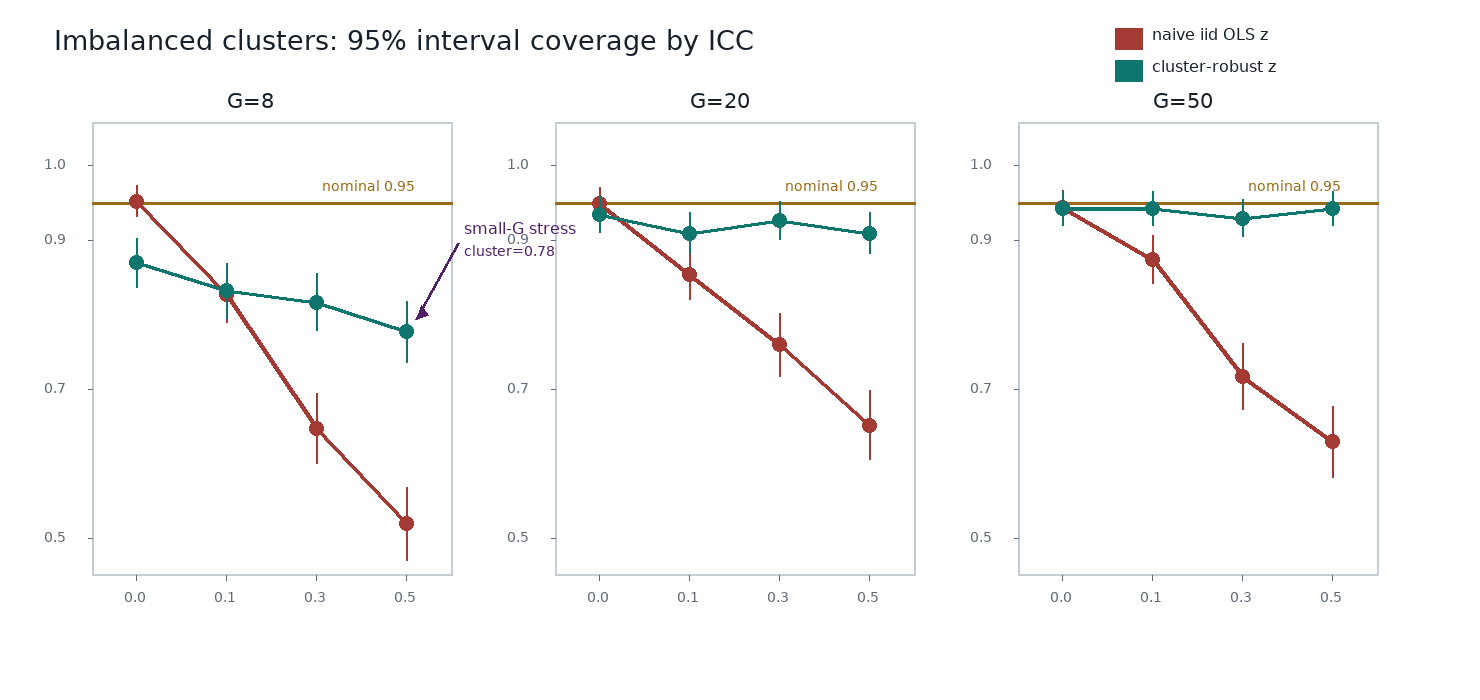
\includegraphics[width=0.6600\paperwidth,height=0.3600\paperheight,keepaspectratio]{stage3_assets/coverage_by_icc.png}};
\StageThreeNode{0.0600}{0.3460}{0.1950}{left}{\small Nominal 0.95 remains visible; the stress point is the small-center setting.};
\StageThreeNode{0.2800}{0.7310}{0.6600}{left}{\scriptsize Synthetic clustered-data example; intervals compared on coverage, width, and bias.};
\end{tikzpicture}
\end{frame}

\section{Design}
\begin{frame}[t]{Simulation varies clustering before interval procedures are compared}
\begin{tikzpicture}[x=\paperwidth,y=-\paperheight]
\path[use as bounding box] (0,0.12) rectangle (1,0.82);
\StageThreeBox{0.1128}{0.4847}{0.2841}{0.5897};
\StageThreeNode{0.1208}{0.5117}{0.1553}{center}{\footnotesize DGP knobs};
\StageThreeBox{0.3021}{0.4847}{0.4734}{0.5897};
\StageThreeNode{0.3101}{0.5117}{0.1553}{center}{\footnotesize Clustered samples};
\StageThreeBox{0.4914}{0.4847}{0.6627}{0.5897};
\StageThreeNode{0.4994}{0.5117}{0.1553}{center}{\footnotesize Interval procedures};
\StageThreeBox{0.6807}{0.4847}{0.8520}{0.5897};
\StageThreeNode{0.6887}{0.5117}{0.1553}{center}{\footnotesize Coverage diagnostics};
\StageThreeArrow{0.2881}{0.5372}{0.2961}{0.5372};
\StageThreeArrow{0.4774}{0.5372}{0.4854}{0.5372};
\StageThreeArrow{0.6667}{0.5372}{0.6747}{0.5372};
\StageThreeNode{0.1128}{0.7635}{0.7392}{left}{\small The connector direction encodes data generation before interval estimation and coverage diagnostics.};
\end{tikzpicture}
\end{frame}

\section{Failure}
\begin{frame}[t]{Small-G settings remain anti-conservative after robustification}
\begin{tikzpicture}[x=\paperwidth,y=-\paperheight]
\path[use as bounding box] (0,0.12) rectangle (1,0.82);
\StageThreeNode{0.1040}{0.3628}{0.7568}{center}{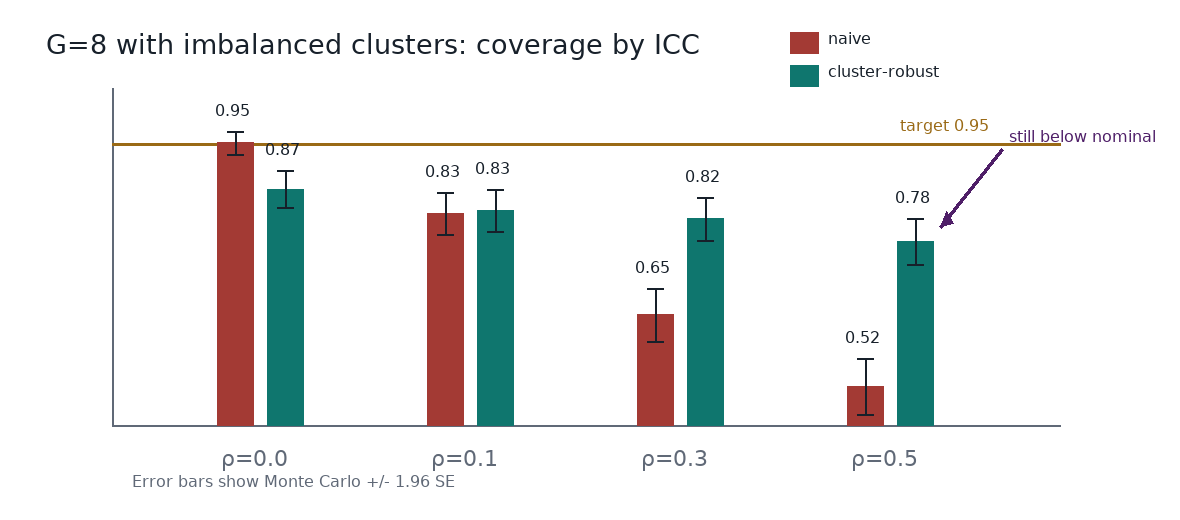
\includegraphics[width=0.7568\paperwidth,height=0.3600\paperheight,keepaspectratio]{stage3_assets/small_g_negative_result.png}};
\StageThreeNode{0.1040}{0.7478}{0.7568}{left}{\small The failure region is adjacent to the diagnostic explanation instead of hidden in a note.};
\StageThreeNode{0.1040}{0.7478}{0.7568}{left}{\scriptsize Negative evidence is completed; CR2 and wild cluster bootstrap remain the next test.};
\end{tikzpicture}
\end{frame}

\section{Medical Image}
\begin{frame}[t]{Same-case panels keep the segmentation error interpretable}
\begin{tikzpicture}[x=\paperwidth,y=-\paperheight]
\path[use as bounding box] (0,0.12) rectangle (1,0.82);
\StageThreeNode{0.0864}{0.3559}{0.1802}{center}{\scriptsize\textbf{Input}};
\StageThreeNode{0.0864}{0.3839}{0.1802}{center}{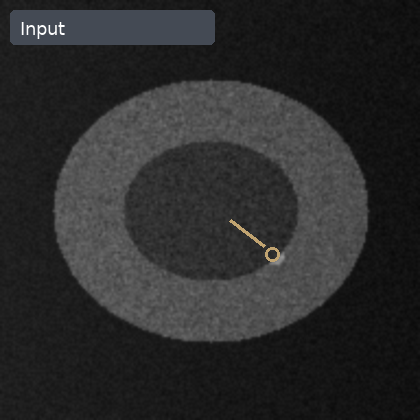
\includegraphics[width=0.1802\paperwidth,height=0.2128\paperheight,keepaspectratio]{stage3_assets/failure_input.png}};
\StageThreeNode{0.2786}{0.3559}{0.1802}{center}{\scriptsize\textbf{GT}};
\StageThreeNode{0.2786}{0.3839}{0.1802}{center}{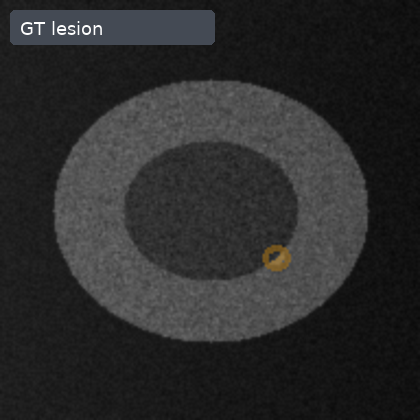
\includegraphics[width=0.1802\paperwidth,height=0.2128\paperheight,keepaspectratio]{stage3_assets/failure_gt.png}};
\StageThreeNode{0.4708}{0.3559}{0.1802}{center}{\scriptsize\textbf{Prediction}};
\StageThreeNode{0.4708}{0.3839}{0.1802}{center}{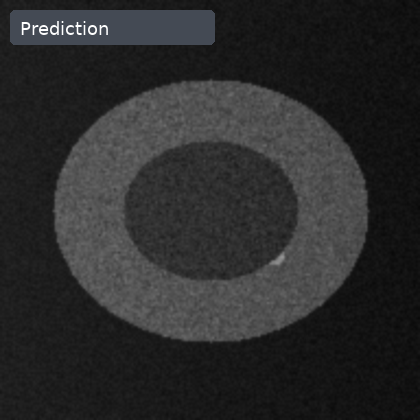
\includegraphics[width=0.1802\paperwidth,height=0.2128\paperheight,keepaspectratio]{stage3_assets/failure_pred.png}};
\StageThreeNode{0.6630}{0.3559}{0.1802}{center}{\scriptsize\textbf{Error}};
\StageThreeNode{0.6630}{0.3839}{0.1802}{center}{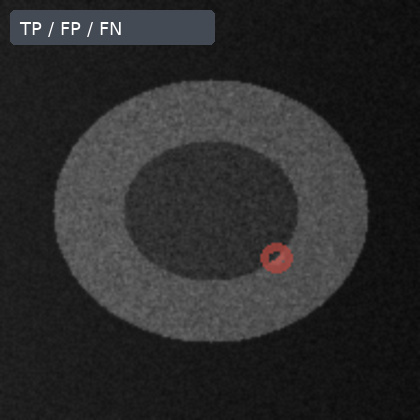
\includegraphics[width=0.1802\paperwidth,height=0.2128\paperheight,keepaspectratio]{stage3_assets/failure_error.png}};
\StageThreeNode{0.0864}{0.6639}{0.7568}{left}{\scriptsize All four panels come from the same case; the error panel binds the failure explanation.};
\end{tikzpicture}
\end{frame}

\section{Next}
\begin{frame}[t]{Next experiment tests whether batch selection reduces fragile coverage}
\begin{tikzpicture}[x=\paperwidth,y=-\paperheight]
\path[use as bounding box] (0,0.12) rectangle (1,0.82);
\StageThreeBox{0.1480}{0.4901}{0.3061}{0.5951};
\StageThreeNode{0.1560}{0.5171}{0.1421}{center}{\footnotesize Small-G limit};
\StageThreeBox{0.3241}{0.4901}{0.4822}{0.5951};
\StageThreeNode{0.3321}{0.5171}{0.1421}{center}{\footnotesize DPP batch query};
\StageThreeBox{0.5002}{0.4901}{0.6583}{0.5951};
\StageThreeNode{0.5082}{0.5171}{0.1421}{center}{\footnotesize Mondrian partition};
\StageThreeBox{0.6763}{0.4901}{0.8344}{0.5951};
\StageThreeNode{0.6843}{0.5171}{0.1421}{center}{\footnotesize CR2 / wild bootstrap};
\StageThreeArrow{0.3101}{0.5426}{0.3181}{0.5426};
\StageThreeArrow{0.4862}{0.5426}{0.4942}{0.5426};
\StageThreeArrow{0.6623}{0.5426}{0.6703}{0.5426};
\StageThreeNode{0.1480}{0.7635}{0.6864}{left}{\small Coverage evidence determines which batch-query strategy to validate next; CR2 and wild bootstrap remain proposed comparators.};
\end{tikzpicture}
\end{frame}

\end{document}
